\section{le réseau de neurones}
Nous avons le regret d'annoncer que notre reseau de neuronne n'est pas fonctionel
néanmoins nous avons fait pas mal de recherche la dessus. Tout abords qu'est ce qu'un neurone ? 
\subsection{un neurone}
un neurone, en biologie, se compose de plusieur partie, nous allons nous contenter aux plus simples c'est à dire : l'axone et le noyau. l'axone est le lien qui permettra de relier plusieur neurone entre eux et le noyaux son centre de commande la ou se fera l'action du neurone. Notre reseau de neurone vas donc simuler le fonctionnement d'un neurone.
\begin{figure}[h]
  \center
  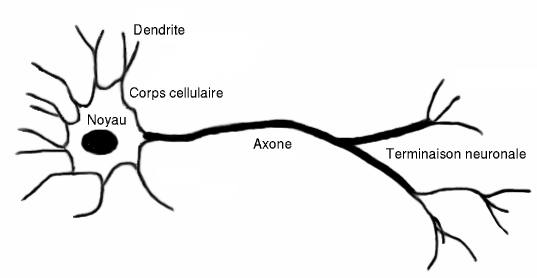
\includegraphics[width=0.80\textwidth]{neurone.png}
  \caption{Un neurone}
\end{figure}
\subsection{un peu d'histoire}
Les reseau de neurone et autre perceptron sont une science a multiple facette qui a connu de nombreux retournement de situation. Ils naissent en 1950 de deux neurologues : Warren McCulloch et Walter Pitts.
\subsection{ce que compose notre reseau de neurone}
\subsubsection{le neurone}
Nous allons donc simuler un neurone formel par : 
\begin{itemize}
\item un poids 
\item une valeur 0 ou 1 
\item un seuil
\end{itemize}
\begin{figure}[h]
  \center
  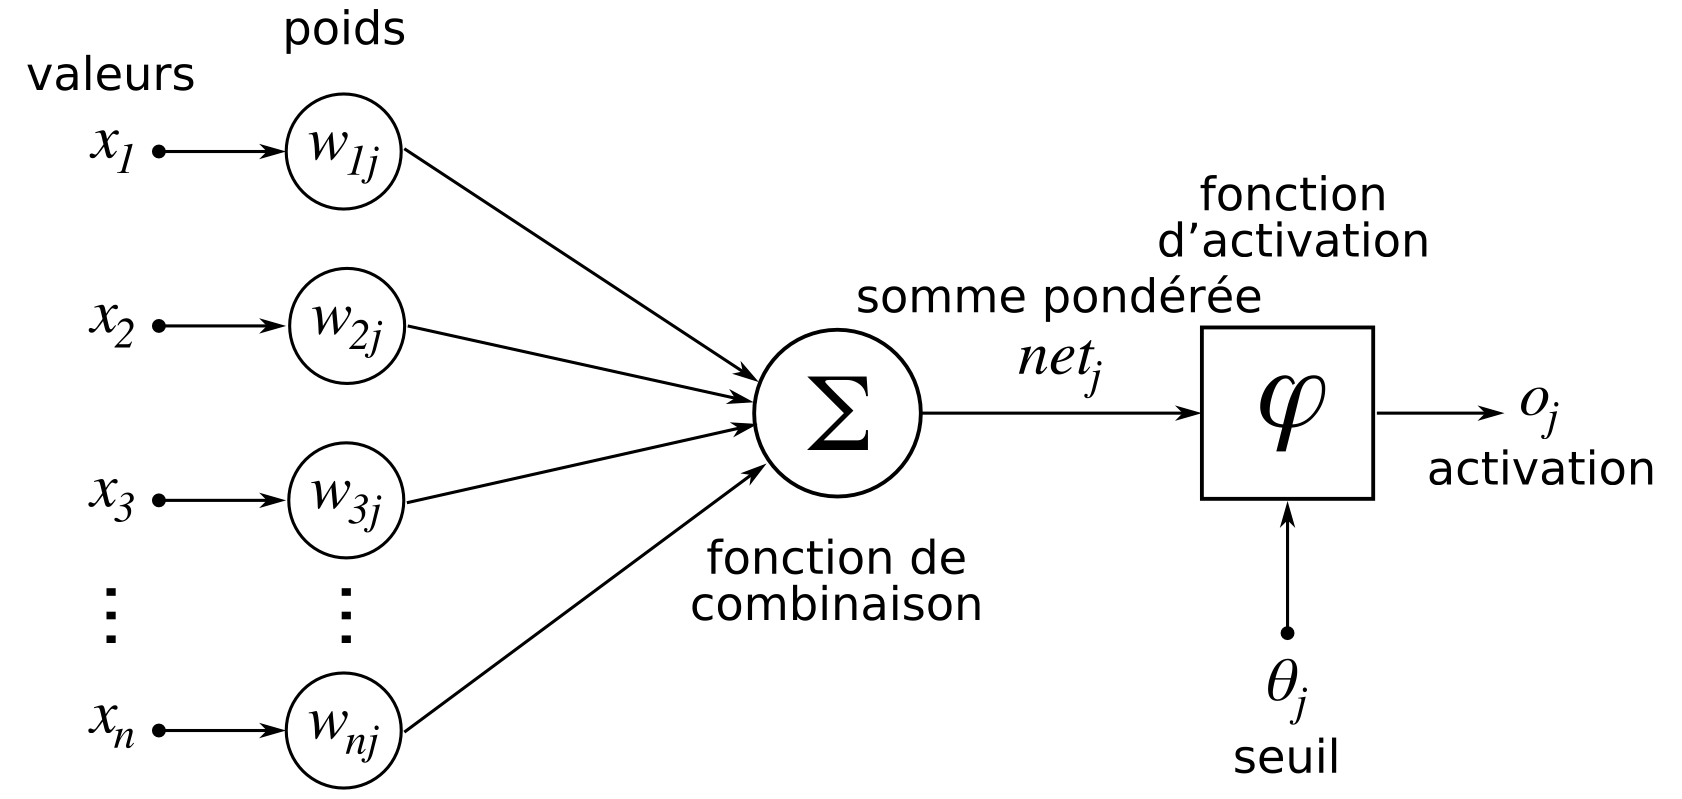
\includegraphics[width=0.80\textwidth]{neuroneformle.png}
  \caption{notre neurone formle}
\end{figure}
Le poids sera la "niveau" de notre neurone c'est lui qui decidera si le neurone va être actif ou non, il pêse (jeux de mot) vraiment dans le réseau de neurone.\\
Sa valeur 0 ou 1 nous travaillons en flottant pour une meilleur valeur de comparaison avec son seuil et sa valeur quand on la passe dans notre fonction sigmoïde (que nous verrons un peu plus loin.\\
Et finallement son seuil qui determinera si le neroune vaux 1 ou 0. Le poids sera comparer à la sigmoïde de 
\subsubsection{la fonction d'activation}
Pour un reseau de neurone il existe plusieur fonction d'activation qui sont :
\begin{itemize}
\item sigmoïde
\item tangente hyperboliqe
\item Heaviside
\end{itemize}
\vspace{0.5cm}
Nous avons choisis d'implementer la fonction sigmoïde car plus partique pour la méthode d'apprentissage par retropropagation.
Mais faisons tout de même un bref tour d'horizon pour justifer ce choix :
\begin{itemize}
\item
La fonction Heaviside est une fonction discontinue tel que :
\begin{center}
[\
  \forall x \in R, H(x) =  0 si x < 0 H(x) = 1 si x >= 0
 \]
\end{center}
La fonction n'est pas dérivable est pose donc un porblème.
\item
La fonction tangente hyperbolique caractériser par :
\begin{center}
\[ th(x) = \frac{e^{x} - e^{-x}}{e^{x} + e^{-x}}\]
\end{center}
\item
Mais nous avons choisis la fonction sigmoïde qui se "rapproche" un peu de la tangente hyperbolique mais la dérivé est nettement plus simple et plus facile à manier que la tangente hyperbolique. La fonction sigmoïde est representé par :
\begin{center}
\[ f(x) = \frac{1}{1 + e^{-x}} \]
\end{center}
L'avantage majeur de cette fonction est qu'elle utilisé en porbabilité logistique et permet de repartir equitablement l'ensemble des poids concernés car l'esperence d'obtenir la moyenne est de 0, ce qui correspond a un équité entre toute les valeurs de poids de notre reseau de neurone dans une couche donné.
Deplus sa dérivé est facilement calculable et vaux
\begin{center}
\[ f(x) = \frac{e^{-x}}{1+e^{-x}} \]
\end{center}
Nous verrons a quoi sert sa dérivé par la suite.
\end{itemize}

\subsubsection{la fonction de seuil}
Une fois nous avons appliquer notre sigmoïde sur les poids menant a un pixel on test si le resultat est superieur au seuil de notre neurone qui est choisis aléatoirement.
Si le resultat depasse le seuil alors le neurone vaut 1 sinon il vaut 0.

\subsection{Algorithmique}
Passon a la mise en pratique de toute ces formules.
L'algorithme prend en paramètre une matrice qui represente un caractère. Donc une matrice de 9x9 (choix arbitraire).
 Notre réseau de neurone possède ainsi 81 entrées. Nous appliquons donc chaque cellule de notre matrice a une entré de notre reseau de neurone.
Nous initialisons l'ensemble des neurones du réseau a 0 et un poids tiré au hasard, car comme chacun sait tout le monde ne démarre pas ave le même cerveau.
C'est alors que la magie opère, nous allons calculer la valeur de chaque neurone de la couche suivante a partir des poids et des valeurs des neurones précédants.
\[ x_{i} = g(\sum_{j} x_{j} w_{ji}) \]
$x_{i}$ est la valeur de neurone i dans la couche suivante\\
$g$ la fonction sigmoïde\\
$x_{j}$ la valeur du neurone j dans la couche \\
$w_{ij}$ le poids qui permet de passer du neurone $x_{j}$ à $x_{i}$\\

On obtien donc pour chaque neurone $x_{i}$ une valeur que l'on va comparé avec le seuil de ce même neurone pour savoir si on va le mettre à 1 ou a 0. On répète ainsi cette action sur toutes les couches jusqu'à la derniere.
\\
Mais comment cela fonctionne-t-il ? C'est alors que pour la deuxieme fois la magie opère. Car nous voulons reconnaitre des inputs pour en tirer un résultat. C'est alors qu'arrive la rétropogation de l'érreur.

\subsection{l'apprentissage}

Il existe plusieurs types d'apprentissage et nous avons choisis la rétropropagation de l'erreur.
Nous allons donc faire apprendre des motifs a notre réseau de neurone. Pour cela on va lui faire faire un apprentissage.
 Notre algorithme va prendre en paramètre un état initial défini et un état final, celui qui doit correspondre à  l'état inital.
Nous allons parcourir le réseau de neurone comme vu précédament et ainsi obtenir une sortie. 
Nous comparons alors notre sortie à notre état final voulu.
Deux choix s'offre à nous : ils sont égaux et alors la c'est gagné ! ca veux dire que les poids sont bien équilibré pour reconnaitre notre motif d'entré.
Sinon on part pour un rééquilibrage des poids. A ce moment la entre en scène notre charmante dérivé de fonctoin sigmoïde qui va nous premettre de faire varier les poids (dérivé... variation... variation.. dérivé... ca ne fait rire que moi...).
Tot d'abord nous calculons l'erreur sur la dernière couche grâce a :
\[e_{i} = g'(\sum_{i}w_{ji}x_{i})(s_{i}-y_{i})\]
$s_{i}$ la valeur du neurone i sur notre sortie voulue\\
$y_{i}$ la valeur du neurone i sur notre sortie obtenue\\
$w_{ij}$ le poids entre le neurone i et son prédéceseur j\\
$x_{i}$ la valeur de notre neutrone i sur la couche actuel\\
$e_{i}$ l'erreur commise.
Et nous pouvons ainsi rétropopagé cette erreur et mettre à jour les poids grâce a\[e_{j} = g'(\sum_{j} x_{j} w_{ji})\sum_{i}w_{ij}e_{i}\]
$e_{j}$ l'erreur sur la couche suivante 
$g'$ la dérivé de la fonction sigmoïde
$x_{j}$ la valeur du neurone j sur la couche précédante
$w_{ij}$ le poid entre le neurone j de la couche précédante et du neurone i de la couche courante
$e_{i}$ l'erreur sur la couche courante.

Une fois que l'on a calculer les différentes érreurs on peut mettre a jour les poids 
\[ w_{ij} = w_{ij} - \lambda e_{i} x_{j}\]
$e_{i}$ l'erreur sur la couche 
$\lambda$ le coefficient d'apprentissage comprise entre 0 et 1 
$x_{j}$ la valeur du neurone j sur la couche precedante.

C'est alors que tou les poids rééquilibrer on peut rélancer un parcours de notre reseau de neurone avec les même paramètre et recommence la retropropagation tant que la couche de sortie n'est pas égale à la couche désiré.

Voila l'apprentissage pour une valeur. Pour plusieure on prend une batterie de test et on la lance jusqu'à ce que tout les test soit concluant les un après les autres.

\subsection{ce qui ne marche pas avec notre réseau de neurone}
L'apprentissage ne se déroule pas bien, impossible de vraiment savoir pourquoi peut être un problème de sur-apprentissage...

